%%!TEX root=../main.tex

\section{Realted work}
\subsection{Localization Algorithm}
In the wireless sensor networ \cite{han2013localization}, the localization is one of the most important topics, because of the widely used in our daily life. The localization algorithms could be separated into two categories: range-free and range-based. The range-free algorithms are using landmarks to connect the unknown nodes, during this process, the information may need the artificial or the GPS system to require. The principle of range-based algorithms is using distance or angle to estimate the location of the targets. The common algorithms of range-based are: the time of arrival, the time difference of arrival, the angle of arrival and received signal strength indication. 

Concerning range-based localization algorithms\cite{kaune2012accuracy}, the time-based algorithms have been widely proposed in the application of different scenarios. The algorithm is using signal propagation time measurement and known propagation velocity to determine the distance between the sensor nodes. The major difference between ToA and TDoA algorithm is the nodes and receivers of ToA should be synchronized. Both the ToA and TDoA algorithms have high accuracy, but the energy-consuming is expensive at the same time. Besides, better performance of hardware is required by the TDoA. 

Comparing to ToA and TDoA, the RSSI\cite{laaraiedh2011comparison} \cite{mistry2015rssi} algorithm could save more energy and cost-effective. The RSSI algorithm relies on the transmitted signal power decays with distance. There is a path loss called free-space propagation loss related to the distance when the nodes sent a signal to the medium. The landmark could calculate the distance between the unknown node and itself by using this relationship. The most typical model between the attenuation of radiofrequency signal and distance in the air is the free space propagation model of radiofrequency signal, based on the Friis transmission equation we could have:\\
\begin{equation}
    \frac{P_{r}}{P_{t}} = \frac{A_{t} A_{r}}{d^{2} \lambda^{2}}
\end{equation}
where the $P_{r}$ represents the power at the receiving antenna, $P_{t}$ means the output power of transmitting antenna, $\lambda$ is the wavelength and d is the distance between the antennas.

The gain of the transmitting antenna could be written as:\\
\begin{equation}
 G_{t} = \frac{4 \pi A_{t} }{\lambda^{2}}
\end{equation}
Then the gain of the receiving antenna could be written as:\\
\begin{equation}
 G_{r} = \frac{4 \pi A_{r} }{\lambda^{2}}
\end{equation}
Since the Effective Isotropic Radiated Power of RF tag is:\\
\begin{equation}
 P_{EIRP} = P_{t}G_{t}
\end{equation}
Therefore, the attenuation of the radiofrequency signal and distance in free space propagation model could be expressed as:\\
\begin{equation}
 P_{r} = P_{EIRP} G_{r} (\frac{\lambda }{4\pi d})^{2}
\end{equation}
The term $(\frac{\lambda }{4\pi d})^{2}$ is called free space path loss.\\
In dB, the expression of (5) becomes:\\
\begin{equation}
 P_{r}(dBm) = P_{t}(dBm) + G_{t}(dB) + G_{r}(dB) -L_{p}(dB)
\end{equation}
To calculate free-space loss by using the above relation and assuming $G_t =G_r =1$:\\
\begin{equation}
 L_{p}(dB) = 20 log_{10} (\frac{4 \pi d}{\lambda})
\end{equation}
The terms $G_{t}(dB)$ and $G_{r}(dB)$ are clearly gains, when they are positive, the received power increases. And as distance increases, $L_{p}(dB)$ increases, which because of the negative sign, reduces the received power.\\

\subsection{Machine Learning Algorithms}
For traditional RSSI algorithm, it use the free-space path loss formula to compute the distance between the objective and the known nodes. Then use trilateration to compute the location of the objective which is a range-based method. For machine learning algorithms, we use machine learning method to predict the location of the object which replace the trilateration. Therefore, our input only need the receivied power and feed to the model.Then the model will predict the location of the objective. So our method is a kind of range-free method.
\subsubsection{RNN based}
The neural network could be divided into the biological neural networks and artificial neural networks, the latter is the mathematical model that we need to learn to simulate animal neural networks. A common problem in modern data analysis is neural network, which can be classified as a semi-parametric method. There are 27 kinds of neural network models, such as perceptron, Markov chain, artificial neural network, cyclic neural network and so on. 

Recurrent neural network (RNN) \cite{tarwani2017survey} is a kind of recurrent neural network that takes sequence data as input, recursion in the evolution direction of sequence and all nodes (cyclic units) are linked in a chain. The traditional neural network only establishes the weight connection between layers. Compared with the traditional neural network, RNN is a special neural network structure. It is proposed according to the view that "people's cognition is based on past experience and memory". It not only considers the input of the previous moment but also creates a "memory" function of the neural network for all the previous contents. The main structure of the RNN neural network model is shown in Figure \ref{RNN structure}.

\begin{figure}[ht]
\centering
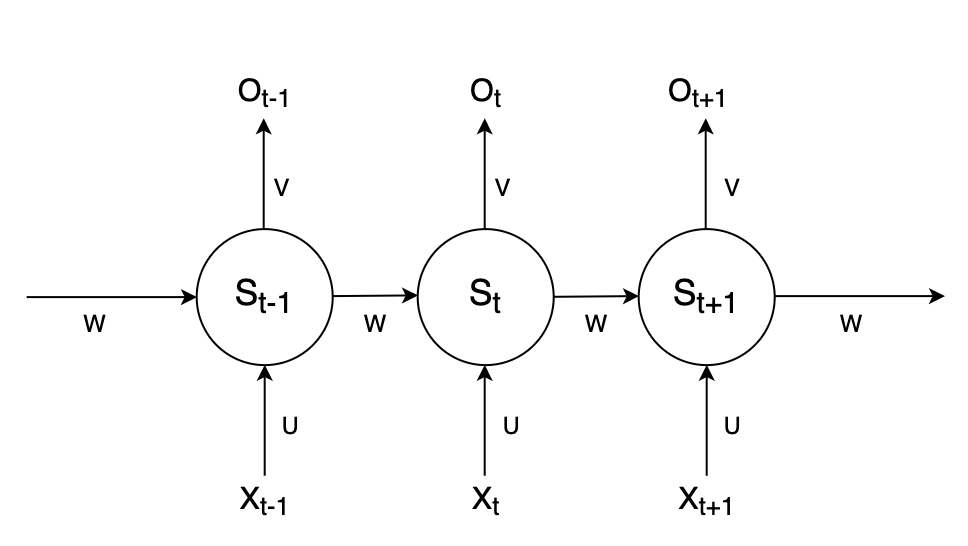
\includegraphics[width=3in]{\FIGDIR/P3_RNN.png}
\caption{The Structure of RNN Model}
\label{RNN structure}
\end{figure}
In the hidden layer of the RNN network, there is an arrow to indicate the circular update of the data and the reverse of the hidden layer. Feedback not only flows into the output, but also flows into the hidden layer of the next time step, and then affects the weight values of the next time step. This is the method to realize the time memory function. The layer by layer expansion diagram of the neural network with multiple time steps is shown in figure.

As shown in the figure, $t-1 $, $t $, $t + 1 $ denotes time series, $x $ represents input samples, $S_ {t} $ is the memory unit of the sample at time T. for the time of $t$, when the sample is input:\\
\begin{equation}
 S_ {t} = f (W S_ {t-1}+ U x_ {t} ) 
\end{equation}

where $W$ is the weight of the input, $u$ is the weight of the input sample at the moment, and $f$ is the activation function.
$O_ {t}$ is the output at the time of $t$:\\
\begin{equation}
O_ {t} = g (V S_{t})    
\end{equation}

Where $V$ is the sample weight of the output and $g$ is the activation function.

The training method of the RNN neural network model is back-propagation through time (BPTT), which continuously searches for better points along the negative gradient direction of parameters to be optimized until convergence. Because of the RNN processes time series, it needs time backpropagation. The weight parameters need to be updated in RNN are W, U and V. If the error value of each output $O_t$ is $e_t$, then the total error can be expressed as: $E = \sum_{t} e_t$.

The cross-entropy loss function or square error loss function could be used as the loss function. Since the output of each step not only depends on the network of the current step, but also needs the network state of the previous steps, the error value of the output end should be transmitted backward, and the gradient descent method is used to update:\\
\begin{equation}
 \Delta U = \frac{\partial E}{\partial U} = \sum_t \frac{\partial e_t}{\partial U}
\end{equation}

\begin{equation}
 \Delta V = \frac{\partial E}{\partial V} = \sum_t \frac{\partial e_t}{\partial V}
\end{equation}

\begin{equation}
 \Delta W = \frac{\partial E}{\partial W} = \sum_t \frac{\partial e_t}{\partial W}
\end{equation}

The advantage of the RNN neural network is that it could effectively deal with nonlinear time series, which makes the previous time-series directly affect the data of the next time point, and the hidden layer of RNN could realize the effect of self-loop recursive feedback. However, RNN is unstable, and gradient vanishing and gradient explosion may occur at any time. The long-term and long-term memory model (LSTM) proposed by Schmiduber et al. (1997) solved the above problems of recurrent neural networks.

As mentioned above, the long and short term memory neural network (LSTM) \cite{smagulova2019survey} \cite{sahoo2019long} is an improvement of RNN. Each layer of LSTM is designed with multiple gate structure neurons, which could memorize any time state of the hidden layer. No matter how long the propagation path of the gradient is, it will not completely disappear or drop to zero. 

The LSTM model has three gates to control each neural unit: an input gate determines when to allow the activation state to pass to the memory unit, an output gate determines whether the activation state leaves the memory unit, and a forgetting gate determines whether the state of the last neuron is completely or partially memorized or completely forgotten. When the gradient decreases, these gates can be used to modify the parameters of the error function of selective memory feedback. The network structure is shown in figure \ref{LSTM}. Each black node is connected with an activation function. The middle node is used to store the internal state of the memory unit. The number of 1 is used as the weight to cross the time step and then feedback to itself. The LSTM network updates the memory unit by recursive equation and activates the mapping from input x to output y: \\

\begin{equation}
i_t = \sigma (W_i x_t + U_i h_{t-1} + V_i c_{t-1} + b_i)
\end{equation}
\begin{equation}
f_t = \sigma (W_f x_t + U_f h_{t-1} + V_f c_{t-1} + b_f)
\end{equation}
\begin{equation}
c_t = f_t \Theta C_{t-1} + i_t \Theta g (W_c x_t + U_c h_{t-1}+b_c)
\end{equation}
\begin{equation}
o_t = \sigma (W_o x_t + U_o h_{t-1} + V_o c_t + b_o)
\end{equation}
where $\sigma$ is the $sigmod$ activation function; $g$ is the tanh activation function; $i$, $f$, $c$, $o$ are the activation vectors of input gate, forgetting gate, cell state and output gate respectively; $W$, $U$, $V$ are the weight matrix; $b$ is the partial value matrix; $\Theta$ is the element by element product of vectors.
The training method of LSTM neural network model also adopts the back propagation algorithm, which is the same as the back-propagation algorithm of RNN. It also updates all parameters by gradient descent method. The difference is that there are two hidden states $h(t)$ and $C(t)$ in LSTM model. Therefore, it is necessary to use gradient descent method for back propagation to update weight parameters.

\begin{figure}[ht]
\centering
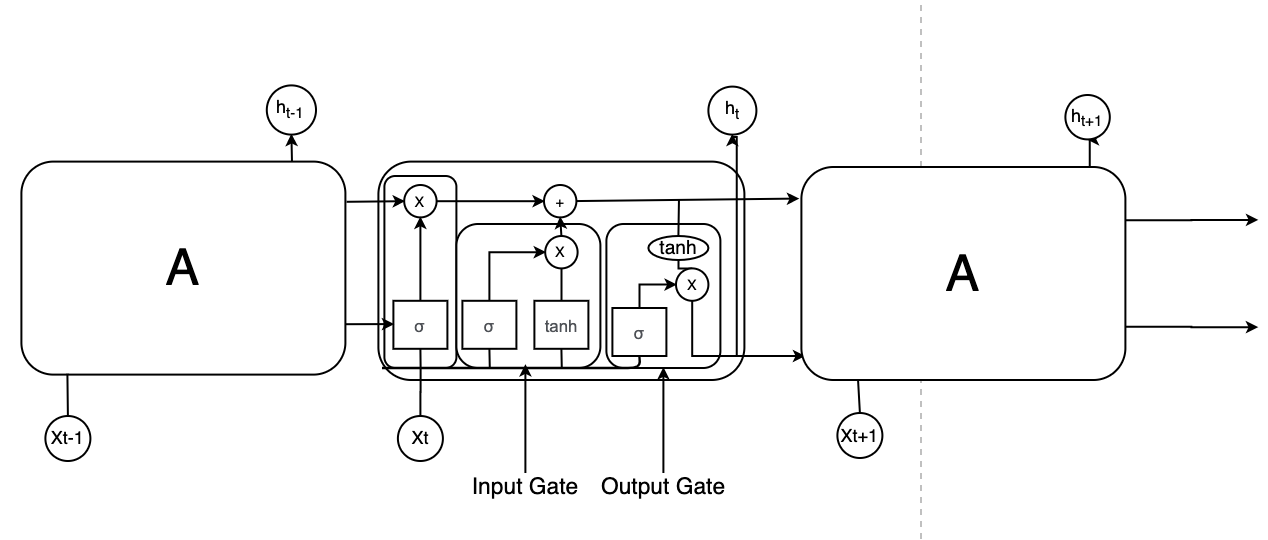
\includegraphics[width=3.5in]{\FIGDIR/P4_LSTM.png}
\caption{The Structure of LSTM Model}
\label{LSTM}
\end{figure}
\subsubsection{MLP based}Another algorithm adopted is Multiple Layers Perceptron (MLP). MLP \cite{taud2018multilayer}  is the fully connected neural network, including the input layer, the output layer and multiple hidden layers. As shown in the figure \ref{MLP}, the layers of the multilayer perceptron are fully connected with each other, and any neuron in the upper layer is connected with all neurons in the lower layer. The hidden layers could be used to solve the non-linear problem. The most simple MLP model contains only one hidden layer, forming a three-layer structure. 

The input layer decided by the number of the dimensions for the vectors. If you have n-dimensional vectors then you have n neurons. Since the neurons in the hidden layer are fully connected to the input layer, assuming that the input layer is represented by the vector x, then the output of the hidden layer would be $f(w_1x+b_1)$, where $w_1$ is the weight, and the $b$ represents the bias, and the function $f$ could be the commonly used Sigmoid function or tanh function. 

About the output layer, from the hidden layer to the output layer can be seen as a multi-category logistic regression, so the output of the output layer is $softmax (w_2 X_1 +b_2)$, where the $X_1$ represents the output $f(w_1X + b_1)$ of the hidden layer. 

\begin{figure}[ht]
\centering
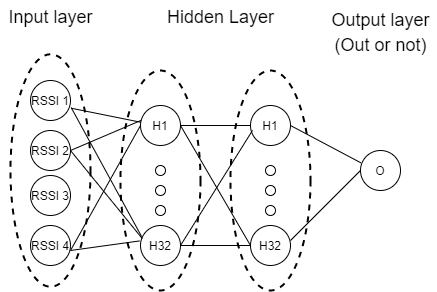
\includegraphics[width=3in]{\FIGDIR/P5_MLP.png}
\caption{The Structure of MLP Model}
\label{MLP}
\end{figure}

\subsubsection{SVM based}
SVM is a supervised machine learning method,the main principle of it is that for linear data, it will find a hyper-plane to separate different classes and maximum the geometric spacing of each. It could also efficiently perform a non-linear classification by using kernel which will implicitly inputs into high-dimensional feature spaces in order to make the data linear.In addition, compared with RNN or MLP, it is more lightweight than those neuron networks so it could easily be deployed on a limited-source equipment,such as wireless sensors.

